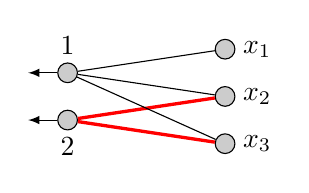
\begin{tikzpicture}[>=latex]
    \tikzset{
        graph-vert/.style 2 args = {
            draw,
            circle,
            inner sep = 0pt,
            minimum size = 0.25cm,
            fill = black!20
        }
    }
    
    \foreach \i in {1, 2, 3}{
        \node[graph-vert] (b\i) at (2, 1.5 - 0.6 * \i) {};
        \node[right = 3pt] at (b\i) {$x_{\i}$};
    }

    \foreach \i in {1, 2}{
        \node[graph-vert] (a\i) at (0, 0.6 * \i - 0.6) {};
        \draw[->] (a\i) -- ++(-0.5, 0);
    }

    \draw[very thick, red] (a1) -- (b3);
    \draw[very thick, red] (a1) -- (b2);
    \draw (a2) -- (b1);
    \draw (a2) -- (b2);
    \draw (a2) -- (b3);

    \node[above = 3pt] at (a2) {$1$};
    \node[below = 3pt] at (a1) {$2$};
\end{tikzpicture}